\section{Results}

\subsection{Nuclear Material Inventory}

\Cref{tab:sim_result1} lists \gls{EU} material inventory in 2050.
The materials continue to accumulate after 2050, but the
\gls{UNF} France receives before 2050 is most impactful for the
feasibility of the transition.


\begin{table}[h]
	\centering
%	\scalebox{0.86}{
	\caption{Nuclear material inventory in the \gls{EU} in 2050 is
                  summarized. The \gls{UOX} in the simulation is either stored or reprocessed to create \gls{MOX}.}

		\begin{tabular}{lrl}
			\hline
			\textbf{Category} & \textbf{Value [MTHM]} & Specifics \\ \hline
			UOX Loaded  & 161,893 & UOX that is loaded into the reactors until 2050 in all EU nations \\ 
			MOX Loaded  & 6,946  & MOX that is loaded in to the reactors until 2050 in all French reactors \\ 
			\textbf{Used UOX Available for Reprocessing (EU except France)}  & \textbf{95,193}  & Used UOX from all EU nations (except for France) that is stored to be reprocessed for ASTRID MOX production.\\
			\textbf{Used UOX Available for Reprocessing(France)} & \textbf{10017}  & Used UOX from all EU nations (except for France) that is stored to be reprocessed for ASTRID MOX production. \\
			\textbf{Reprocessed French UOX} & 53,601 & French used UOX that has already been reprocessed for the production of LWR MOX \\
			Tails  & 980,289  & (Tails generated) $-$ (Tails used for production of LWR MOX) \\ 
			Natural U Used  & 1,142,182  & \\ \hline
		\end{tabular}
		
		\label{tab:sim_result1}
\end {table}
\FloatBarrier


Figures \ref{fig:eu_tail} and \ref{fig:eu_snf} show the 
accumulation of tails and used fuel over time in the \gls{EU}.
Tails accumulate as a by-product of uranium enrichment. For every
ton of \gls{UOX} fuel, about nine times of tails is produced. 
Spent fuel is discharged from reactors every refueling period.
The entire core is discharged when the reactor decommissions.
A total of about $1,000,000$MTHM of tails and $100,000$MTHM of
\gls{UNF} have accumulated by 2050.
Figure \ref{fig:eu_fuel} shows the amount of fuel used in the \gls{EU}.


\begin{figure}[htbp!]
	\begin{center}
		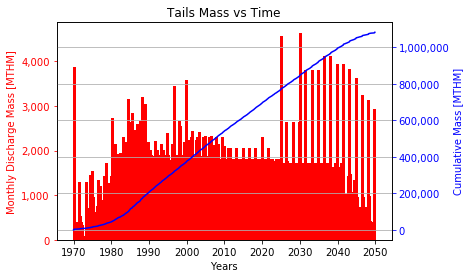
\includegraphics[scale=0.7]{./images/eu_future/tails.png}
	\end{center}
	\caption{This plot shows the timeseries of tails mass accumulation and discharge in the \gls{EU} nations.
			 Tails mass accumulation is fairly steady, with peaks occurring when
			 new reactors are deployed.}
	\label{fig:eu_tail}
\end{figure}

\begin{figure}[htbp!]
	\begin{center}
		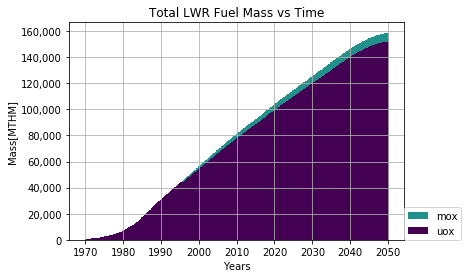
\includegraphics[scale=0.7]{./images/eu_future/total_fuel.png}
	\end{center}
	\caption{This plot shows the timeseries of total fuel usage in the \gls{EU} nations.}
	\label{fig:eu_fuel}
\end{figure}


\begin{figure}[htbp!]
	\begin{center}
			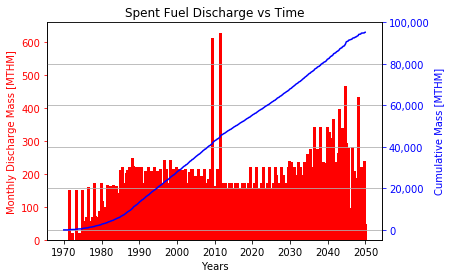
\includegraphics[scale=0.7]{./images/eu_future/snf_discharge.png}
	\end{center}
	\caption{This plot displays the timeseries of \gls{UNF} accumulation and discharge in the \gls{EU} nations.
			 The peaks are caused by decommissioning of reactors, where all the core is sent to the repository.}
	\label{fig:eu_snf}
\end{figure}
\FloatBarrier


\begin{table}[h]
	\centering
	\caption{Plutonium from \gls{UNF} inventory.}
	\begin{tabular}{lrr}
		\hline
		\textbf{Isotope} & \textbf{Mass Fraction in Used Fuel [\%]} & \textbf{Quantity [t]} \\ \hline
		Pu238 & 0.0111 & 10.52109 \\ 
		Pu239 & 0.518 & 544.9927 \\ 
		Pu240 & 0.232 & 244.089 \\ 
		Pu241 & 0.126 & 132.565 \\ 
		Pu242 & 0.0487 & 51.237 \\ \hline
		\textbf{Total} & \textbf{0.9358} & \textbf{983.4} \\ \hline
	\end{tabular}
	
	\label{tab:pu}
\end{table}



\subsection{French \gls{SFR} Deployment}

Reprocessing \gls{UNF} collected from all EU nations can start approximately
180 \glspl{SFR}. Table \ref{tab:pu} lists the isotope, mass fraction,
and quantity of plutonium that can be obtained from the 2050 \gls{UNF} inventory.
 With the \gls{SFR} breeding ratio above one, France can transition into
a fully \gls{SFR} fleet without extra construction of \glspl{LWR}. 

From Varaine et al. \cite{varaine_pre-conceptual_2012}, a French
ASTRID-type 600\gls{MWe} \gls{SFR} consumes $1.225$ metric tons of
plutonium a year, with an initial plutonium loading of $4.9$ metric tons. 
Thus, the number of \glspl{SFR} that can be loaded with the reprocessed
plutonium from \gls{UNF} can be estimated to be 249, assuming infinite 
reprocessing and fabrication capacity as well as abundant depleted uranium 
supply.
 
Used \gls{MOX} from an ASTRID reactor is 23.95\% plutonium
in this simulation (see \cref{tab:comp}), whereas a fresh \gls{MOX} is 22\% plutonium.
The plutonium breeding ratio in this simulation is thus assumed to be
$\approx 1.08$.

\Cref{fig:fuel} shows \gls{MOX} loaded in the \glspl{SFR} per month.
The spikes are due to initial fuel demand for new deployment of \glspl{SFR}.
The initial loading of new \glspl{SFR} are done with the \gls{MOX} created
from legacy \gls{UNF}. Once the deployed \glspl{SFR} create enough amounts
 of extra plutonium, the legacy \gls{UNF} is no longer used. 

\begin{figure}[htbp!]
	\begin{center}
		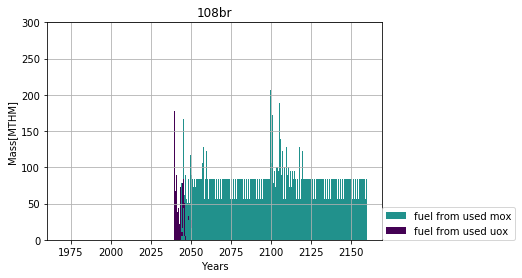
\includegraphics[scale=0.7]{./images/french-transition/where_fuel.png}
	\end{center}
	\caption{This plot shows the timeseries of fuel loaded into \glspl{SFR}.
			 The plot has peaks during a period of aggressive deployment of \glspl{SFR}
			 followed by an equilibrium at 150 \gls{MTHM}. The peaks reoccur with the
			 deployment of the second generation of \glspl{SFR}.}
	\label{fig:fuel}
\end{figure}


 \Cref{fig:pu_no_cum} shows the separated plutonium discharge
per month from the reprocessing plant. The plutonium outflux
does not precisely follow the fuel demand because \Cyclus agents have
material buffers that store commodity fuel for later usage. The reprocessed
plutonium from legacy \gls{UNF} is stored for the initial loading of \glspl{SFR}.
\Cref{tab:sfr_sim_result} lists metrics obtained from the second simulation.

\begin{figure}[htbp!]
	\begin{center}
		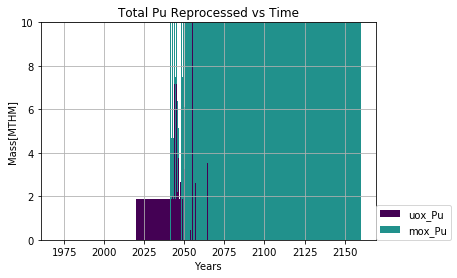
\includegraphics[scale=0.7]{./images/french-transition/pu.png}
	\end{center}
	\caption{This plot shows the separated plutonium discharge from the reprocessing plant.
			 The reprocessing demand for the first aggressive deployment of \glspl{SFR}
			 are lessened because the plutonium demand is met with plutonium separated from legacy \gls{UNF}.
			 The plutonium from reprocessing legacy fuel is a flat rectangle because the 
			 reprocessing throughput was set to 20 $\frac{\gls{MTHM}}{month}$ to avoid reprocessing
			 all the legacy in one timestep. }
	\label{fig:pu_no_cum}
\end{figure}

\begin{table}[h]
	\centering
	\caption {In the French transition to \glspl{SFR},
				  the total legacy \gls{UNF} reprocessed is the 
                                  amount of \gls{UNF} France needs 
				  for a transition into a fully \gls{SFR} fleet. 
                                  %The tails used is around ninth of the original tails inventory from the previous simulation.
                                  %KDH note: What does this mean?
                                  %thought there was only one simulation. . . 
                          }
	\scalebox{0.86}{
		\begin{tabular}{llr}
			\hline
			\textbf{Category} & \textbf{Unit} & \textbf{Value}  \\ \hline
			Total \gls{ASTRID} MOX used & MTHM & 63,425  \\ 
			\textbf{Average UOX Reprocessing} & MTHM/month & \textbf{107.16} \\
			\textbf{Average Total Reprocessing} & MTHM/month & \textbf{36.60} \\
			\textbf{Average Fuel Fabrication} & MTHM/month & \textbf{93.99} \\
			Total \glspl{SFR} Deployed & & 220 \\ 
			Total Plutonium Reprocessed & MTHM & 15,220 \\ 
			Total \gls{ASTRID} fuel from UOX Waste & MTHM & 2,889  \\ 
			Total \gls{ASTRID} fuel from MOX Waste & MTHM  & 60,535 \\ 
			Total Tails used & MTHM & 49,471 \\ 
			\textbf{Total legacy UNF reprocessed} & MTHM & \textbf{53,492} \\ 
			Total Reprocessed Uranium Stockpile & MTHM & 193,120 \\ 
			Total Raffinate & MTHM & 24,376 \\ \hline
		\end{tabular}}
		
		\label{tab:sfr_sim_result}
\end {table}

Despite the large amount of initial plutonium that has to be reprocessed
prior to \gls{ASTRID} deployment, the 20 years of preparation of
\gls{ASTRID} fuel (2020-2040) allows a reasonable level of average
\gls{UOX} reprocessing capacity demand. \gls{UOX} reprocessing continues 
until 2057, when the \gls{ASTRID} spent fuel can supply the plutonium
for its own fuel.


